% COMP702 CA1 Specification and Design Proposal
% Vaibhav Lalwani (201979723), University of Liverpool
% Target length: about five pages of body (title block excluded).
% Compiles with pdflatex: needs graphicx, geometry, booktabs, enumitem, hyperref.
\documentclass[10.5pt]{article}
\usepackage[a4paper,top=18mm,bottom=16mm,left=20mm,right=20mm]{geometry}
\usepackage[T1]{fontenc}
\usepackage{lmodern}
\usepackage{microtype}
\usepackage{graphicx}
\usepackage{booktabs}
\usepackage{enumitem}
\usepackage[hidelinks]{hyperref}
\usepackage{titlesec}

\setlist{nosep,leftmargin=1.4em}
\titlespacing*{\section}{0pt}{8pt}{3pt}
\titlespacing*{\subsection}{0pt}{6pt}{2pt}
\titleformat{\section}{\normalfont\large\bfseries}{\thesection.}{0.5em}{}
\titleformat{\subsection}{\normalfont\bfseries}{}{0em}{}
\setlength{\parskip}{3pt}
\setlength{\parindent}{0pt}
\renewcommand{\baselinestretch}{1.04}

\title{\vspace{-12mm}\bfseries Kodro: An Offline, Self-Refining Platform for Designing Robots and Validating Their Behaviour in Realistic Simulation}
\author{}
\date{}

\begin{document}
\noindent\raisebox{-3mm}{
\includegraphics[height=11mm]{img/uol_logo.png}}\hfill
{\footnotesize\sffamily\MakeUppercase{University of Liverpool}\\[1pt]Department of Computer Science \,$\cdot$\, COMP702 MSc Project}\\[2pt]
\hrule
\smallskip
\maketitle
\vspace{-16mm}

\begin{center}
\small\itshape Specification and Design Proposal (CA1)
\end{center}
\smallskip

{\small
\textbf{Name:} Vaibhav Lalwani \quad \textbf{Student ID:} 201979723 \quad \textbf{Supervisor:} Keith Dures \quad \textbf{Date:} 19 June 2026\par
\textbf{Ethics:} data category A0, participant category 2. Work to date uses simulated personas only, with no human participants and no personal data. Any later study with real users will be agreed with my supervisor and run under appropriate consent before it begins.\par}

\smallskip
\hrule
\smallskip

{\small\textbf{Abstract.} Kodro is an offline desktop platform on which a non-expert designs a custom robot, programs it in Python, blocks or voice with a grounded local assistant and an automatic code reviewer, and validates its behaviour in a realistic simulated world before building any hardware. The robot the user assembles drives the simulation, so changing the build changes the behaviour. A small language model, run only on the local machine, grounds its suggestions in that build and refines its advice from accumulated use through reflection and a reusable skill library, without retraining the model or reaching the internet. This proposal states the aims and measurable objectives, the literature the design follows from, the implementation approach, the data and ethics position, and an evaluation that separates whether a non-expert builds a better behaving robot with the tool from whether the assistant measurably refines its suggestions as its experience grows.\par}

\section{Project description}
Many people have an idea for a robot and no safe, cheap way to try it. Buying parts, wiring a board and writing control code is slow, and the first time a real robot meets the real world it tends to drive into something. Kodro closes that gap with a single offline download. A user designs a robot in a builder, choosing a chassis, a controller board such as an ESP32 or a micro:bit, and the sensors and motors it carries; programs its behaviour in real Python, in blocks, or by voice, with a grounded assistant and a second agent that reviews the code; then runs it in a world with terrain, physics and other moving agents such as pedestrians and traffic. The user watches the robot behave, fixes it, and runs it again, all before spending anything on hardware.

What makes this a research project rather than a toy is the layer above the simulator. A small model, running locally, helps write and check control code and refines itself as the tool is used: after each run it records what happened, keeps a growing library of behaviours that worked, and draws on that record when helping with the next design. It does this without retraining and without reaching the internet, so a user's designs never leave the machine. The project asks one sharp question: how far can such a system genuinely refine itself, and how trustworthy can its validation be, under a hard offline constraint that rules out the cloud and rules out changing the model's weights.

\section{Aims and objectives}
The aim is a working offline platform on which a non-expert designs a robot, programs it, and validates that behaviour in a realistic, agent-populated simulation before building it. Each objective below carries a plain test of done so progress is judged, not asserted.

\textbf{Core objectives (the artefact must achieve these to be a working platform).}
\begin{itemize}
\item Let the user design a robot from a board, sensors and actuators, where the specification drives the simulation. Done when changing the build changes behaviour: a heavier robot drains its battery faster, a stronger motor raises top speed, and a fitted sensor unlocks its command while an absent one withholds it.
\item Execute the robot's real Python in a sandbox that blocks file, network and process access, and score every run against the scenario's success criteria. Done when a hostile program cannot reach the disk and a correct one is scored correctly.
\item Run the robot in a world with terrain, physics and moving agents, across repeated randomised runs. Done when one program runs over several seeds and returns a report of successes, collisions and time to goal.
\item Run the assistant on a local model only, grounded in the robot's specification, and fall back to deterministic rule-based behaviour within two seconds when no model is present. Done when the platform is fully usable with the network off and no model installed, and when the model cannot call a part the build lacks.
\item Refine suggestions from use without retraining, through reflection retrieval and a reusable skill library. Done when, across a session, the system reuses a stored reflection or skill and the median iterations to a working design fall.
\end{itemize}

\textbf{Future-work objectives (beyond the core artefact, attempted only once the above hold).} Broad support for users with particular access needs, such as a full screen-reader path, dyslexia-friendly and low-vision modes, and a study population drawn to include those users, is a stretch goal rather than a core deliverable. The core artefact is specified to produce a working, validated platform first; this wider support is recorded here as an objective for later work so the scope stays honest and achievable within the project window.

\section{Background and key literature}
The design follows from three lines of work rather than sitting beside them. The first is constructionism (Papert, 1980), the durable finding that people learn most when they build something they can watch behave and then debug; Kodro is built around exactly that loop, and a user offers blocks that compile to the same Python so the move from blocks to text needs no change of tool.

The second is why a simulator is worth trusting at all. The central problem in robotics is the gap between simulation and reality, the drop in performance when behaviour tuned in simulation meets the real world. The accepted answer is not a perfect simulator but domain randomization (Tobin et al., 2017): vary friction, mass, sensor noise and the scene across many runs, so behaviour that survives the spread is likely to survive reality. Kodro adopts this directly, validating each design across randomised seeds and reporting the spread, not only the average, and populating its worlds with agents that avoid each other and the robot so a car or home robot is tested among things that move.

The third concerns the model itself and justifies both the offline choice and the careful framing of refinement. Hallucination is intrinsic to these models rather than a patchable bug (Huang et al., 2023), and in generated code it surfaces as plausible but wrong calls (Lee et al., 2025), which is dangerous when the output is control code a beginner cannot tell is wrong. The standard mitigation is to ground generation in retrieved material rather than the model's memory (Lewis et al., 2020); for robots, the model is best constrained to compose a known, safe set of capabilities rather than invent them, in the spirit of programs written against a fixed robot interface (Liang et al., 2023; dos Santos et al., 2026) and of grounding instructions in what the robot can actually do (Ahn et al., 2022). Kodro grounds every suggestion in the build the user assembled, so the model cannot call a sensor that is not fitted; grounding is also why no cloud is needed, since it works on local material. On refinement over time the proposal is deliberately careful: genuine weight-level self-evolution is unsolved (Tao et al., 2024), so Kodro does not claim it. Instead it refines at the level of the system, through a verbal reflection loop (Shinn et al., 2023) and a growing library of behaviours that worked (Wang et al., 2023), composed for new designs without retraining, mirroring recent experience-driven self-evolving agents that improve from their own history without changing weights (Wu et al., 2025). Where several agents cooperate, naive setups fail in characteristic ways (Cemri et al., 2025), which is why a deterministic check, not another model, always has the final word, with an automatic reviewer flagging suspect code before that, following recent automated code-review practice (Sun et al., 2025), and deterministic static analysis can catch hallucinated code outright (Khati et al., 2026).

\section{Design and implementation}
The platform is written in Python 3.12 behind a desktop web view, and each choice follows from the offline, low-resource constraint. The interface is built in React but precompiled to a single bundle, so the panelled layout is kept while the cost of a runtime compiler is paid once at build time. The three-dimensional world uses a copy of the Three.js library held in the project, so the graphics work with the network off. A user's designs and the system's accumulated record are stored in SQLite, a single standard-library file with no server. The assistant calls a local model served by Ollama, which installs as one small application and keeps a model warm with a single command a non-technical user can follow.

The robot is not cosmetic. Its specification is a single source of truth the rest of the system reads: the chosen board, sensors and motors set the mass, which scales battery drain, set the top speed, and decide which commands exist, so a build without an ultrasonic sensor has no distance reading to call and the grounded assistant cannot suggest one. Behaviour is then validated across several randomised seeds with varied friction, mass and sensor noise (Tobin et al., 2017), in worlds that include moving pedestrians and traffic, so a run reports a spread rather than one tidy number.

The model is not used off the shelf. A small open-weight base in the one to three billion parameter range is fine-tuned offline with parameter-efficient QLoRA, using Unsloth and LLaMA-Factory on a single consumer graphics card (an RTX 3050, 6 GB), on the project's own corpus of robot API calls and validated programs, so the resulting model, kodro-coder, speaks the platform's exact command set rather than generic Python. The size is deliberate: it is the largest class that still answers at an interactive pace on a mainstream laptop with no discrete graphics card, where a seven billion model would need a card a school laptop rarely has. Two variants are packaged, a one billion drafter for instant suggestions and a three billion model for quality, both exported to GGUF and served through Ollama; the fine-tune is a one-time development step, and the exported model then runs on the user's machine with no card and no network. Recent work shows small local models with retrieval give reliable, low-hallucination help offline (Reza et al., 2025), and onboard small models are now being shown to drive robot task planning and code generation on constrained hardware (Wang et al., 2026). The honest limit is that this buys domain grounding and a reliable output format, not frontier capability: a small local model cannot match a cloud model, so the design leans on grounding and the simulation gate, not on the model being clever. The fallback is a defined deterministic path that returns rule-based code and checks when no model is present. Refinement is concrete and avoids changing the weights, and is called refinement, not improvement, on purpose. Three local, countable mechanisms carry it: after each run the system writes a short reflection on what failed and worked and retrieves the most similar past reflections into the next suggestion (Shinn et al., 2023); routines that passed validation are kept as named, parameterised skills and composed into later designs (Wang et al., 2023); and a table of past designs and their outcomes is sampled so advice on a new build is anchored in what happened on similar ones. None of this edits the model. The work is built as small, independently tested changes, each merged only after a continuous integration pipeline runs the full test suite, a type checker and a linter, so the codebase stays releasable at every step.

\begin{figure}[t]
\centering
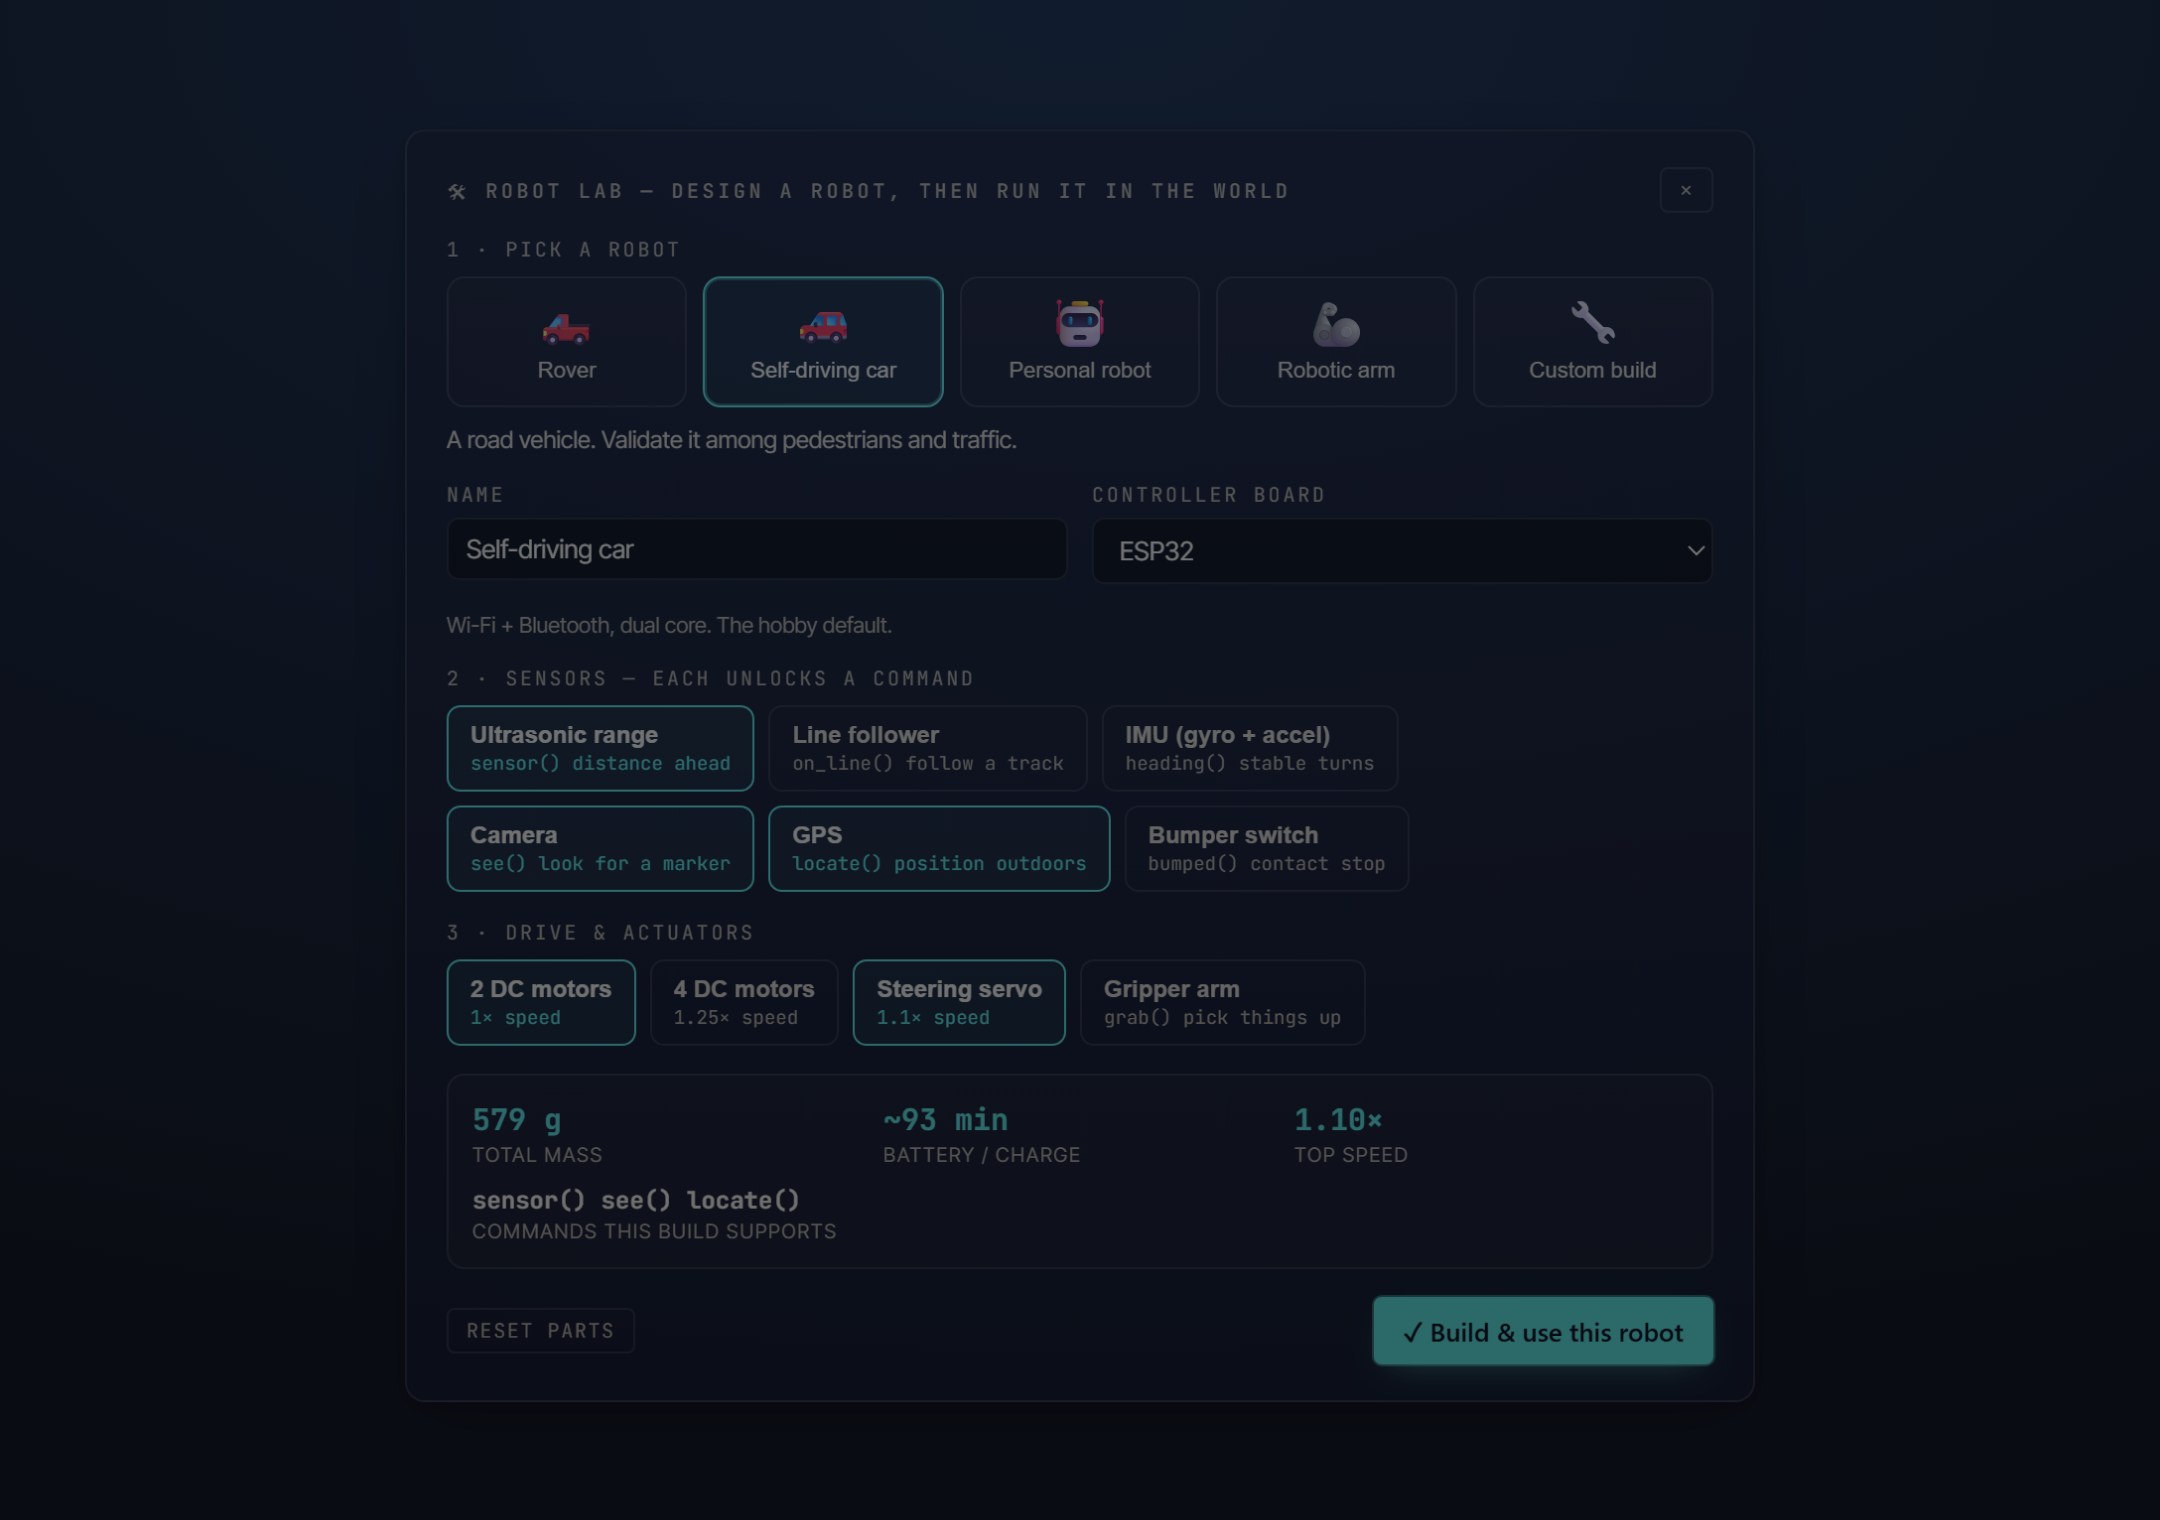
\includegraphics[width=0.78\linewidth]{img/robot_lab.png}
\caption{The Robot Lab. The user designs a custom robot and the build's mass, battery life and supported commands update live; that specification then drives the simulation.}
\end{figure}

\section{Data and evaluation}
The project uses no external datasets and no personal data. Its content is authored by hand as structured files: a set of starter robots and a set of validation scenarios, each a goal plus the criteria that mark success. The only data made at runtime is the user's own designs and code, the per-run results, and the reflections the system writes, all kept in the local file and never sent anywhere; that record is also the substance of the refinement. The local model runs from weights already on the device.

Evaluation separates three questions that must not be blended. \emph{Is it usable?} A panel of distinct simulated personas, generated to span the makers who might use the tool, each drives one session and returns a mark out of ten with the concrete defects it found; after each round the named defects are fixed and the same build is re-rated. This is a low-cost inspection method, useful for breadth and speed and reported with its limit stated plainly: a rising score shows the tool became learnable to drive, which is a usability finding and nothing more. The measured trajectory is below.

\begin{table}[h]
\centering\small
\begin{tabular}{clp{7.2cm}c}
\toprule
Round & Personas & Focus & Mean (/10) \\
\midrule
1 & 50 & First contact with the build & 5.86 \\
2 & 12 & After the first round of fixes & 6.50 \\
3 & 50 & After wiring the learner model and teacher tools into the app & 7.10 \\
4 & 50 & After grounded answers and the voice route were added & 7.36 \\
5 & 8 & Focused review of the new three-dimensional world & 6.40 \\
\bottomrule
\end{tabular}
\end{table}

\emph{Does it help?} A within-subject design study has about sixteen non-experts each attempt two comparable held-out scenarios, one with Kodro's grounded help and reviewer and one without, order counterbalanced. The headline measure is task success in simulation, where a design runs twenty times with friction, mass and sensor noise randomised (Tobin et al., 2017) and passes if it completes the scenario in at least sixteen of twenty; iterations to a working design and collisions are recorded alongside. The analysis, a paired test on success and on iterations, is fixed before any data is collected, and the result is read as exploratory: sixteen is small and the sample is a convenience one, so a positive result is a signal to confirm at scale, not proof. \emph{Does it refine?} The same participant tackles a sequence of related scenarios in two arms whose only difference is the memory: the full arm against an ablated arm with reflection retrieval and the skill library off. The full arm should reach a working design in at least a quarter fewer iterations, and a retrieved reflection should precede a successful next attempt clearly more often than the base rate. The assistant is also measured directly on a fixed set of design questions, including off-specification and adversarial ones: grounded answers must be correct at least eighty-five percent of the time and invent a missing part less than five percent of the time, and grounding must beat the same model asked without the specification. The five percent invention rate is a release gate; above it, only the deterministic path ships.

\section{Ethics, plan and risks}
No human participants have been involved to date; the personas are software and reported as such. The planned study falls under participant category 2, uses adult and older makers, gives a plain explanation, anonymises data at collection, and is agreed with the supervisor under consent before it begins. One risk is specific to the technology and deserves naming: the output is control code for a machine a user may build, so a confident falsehood could drive a real robot into a person or a wall. The design treats this as a safety requirement. Every suggestion is grounded in the build, the assistant refuses and points back to the specification rather than guess, and any code runs first inside the sandboxed simulation and is checked against the scenario, so a wrong suggestion fails visibly on screen rather than on real hardware. The mandatory simulation gate, not the model, stands between a generated program and the world.

\begin{figure}[t]
\centering
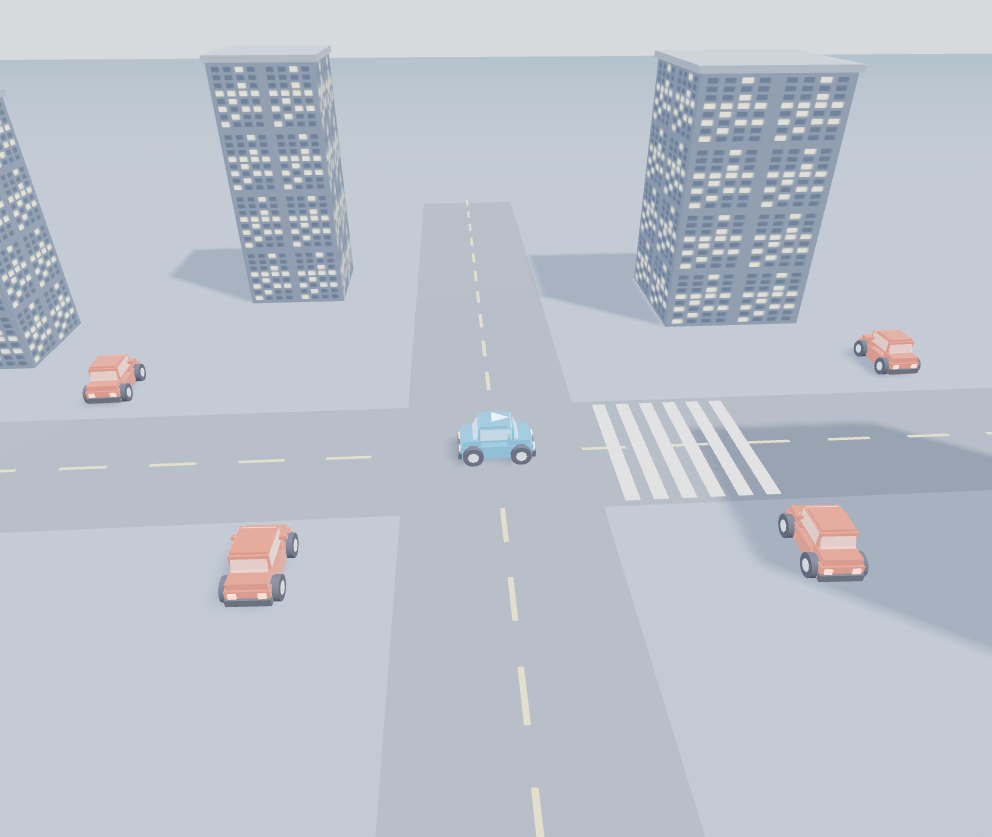
\includegraphics[width=0.78\linewidth]{img/city_3d.png}
\caption{Validation in a realistic world. The designed robot runs in a city street rendered in three dimensions, among traffic and pedestrians that move around it, so its behaviour can be watched before any hardware is built.}
\end{figure}

The plan runs from this proposal to the dissertation, with the demonstration video (CA2) and write-up (CA3) built in and fortnightly supervisor meetings throughout. The critical path runs through ethics approval into the design study and on into the write-up, which is why approval is sought in June with recruiting lead time; the write-up begins during the study on parts that do not need its results, with a buffer before the deadline. The main risks and their contingencies are below. The project is intended to meet the six BCS honours outcomes: it engages current problems (hallucination and grounding, honest offline refinement, the simulation-to-reality gap), justifies its techniques against the literature, and is reported with its weak early results and the fixes that followed rather than only its best numbers.

\begin{table}[h]
\centering\small
\begin{tabular}{p{4.4cm}p{8.2cm}cc}
\toprule
Risk & Contingency & Likelihood & Impact \\
\midrule
Generated control code is unsafe & Every program runs first in the sandboxed simulation against the scenario; grounding and the reviewer catch invented commands before that. & Medium & High \\
Local model too weak for some suggestions & Grounding ties suggestions to the build and the model refuses rather than guesses; a stronger local model can be configured. & Medium & Medium \\
Ethics approval or recruitment delayed & Approval sought in June with lead time; if it slips, the participant-free evaluations run instead and the write-up is not blocked. & Medium & Medium \\
Running out of time & The build is releasable at every step, so an earlier version is always a valid deliverable. & Medium & High \\
\bottomrule
\end{tabular}
\end{table}

Honestly, the originality is not a new algorithm. Retrieval grounding, a sandboxed gate, an experience memory, a skill library and domain randomization are each known, and the offline constraint actively limits how clever any one can be. The contribution is the demonstration that these parts combine into an honest design-and-validation platform that runs entirely on one machine, and a measured account of how far offline self-refinement can go when changing the weights is off the table. The constraint is the point, not a limitation to apologise for.

\section*{References}
{\small\setlength{\parindent}{0pt}\setlength{\parskip}{2pt}
Ahn, M., Brohan, A., Brown, N. et al. (2022) Do as I can, not as I say: grounding language in robotic affordances. \textit{arXiv:2204.01691}.\par
Cemri, M., Pan, M.Z., Yang, S. et al. (2025) Why do multi-agent LLM systems fail? \textit{arXiv:2503.13657}.\par
dos Santos, V.G., Khadraoui, I., Farhat, I. et al. (2026) ALRM: agentic LLM for robotic manipulation. \textit{arXiv:2601.19510}.\par
Huang, L., Yu, W., Ma, W. et al. (2023) A survey on hallucination in large language models. \textit{ACM Transactions on Information Systems} (arXiv:2311.05232).\par
Khati, D., Rodriguez-Cardenas, D., Pantzer, P. and Poshyvanyk, D. (2026) Detecting and correcting hallucinations in LLM-generated code via deterministic AST analysis. \textit{arXiv:2601.19106}.\par
Lee, Y., Song, J.Y., Kim, D. et al. (2025) Hallucination by code generation LLMs: taxonomy, benchmarks, mitigation, and challenges. \textit{arXiv:2504.20799}.\par
Lewis, P., Perez, E., Piktus, A. et al. (2020) Retrieval-augmented generation for knowledge-intensive NLP tasks. \textit{Advances in Neural Information Processing Systems}, 33, pp. 9459 to 9474.\par
Liang, J., Huang, W., Xia, F. et al. (2023) Code as policies: language model programs for embodied control. \textit{IEEE ICRA}.\par
Papert, S. (1980) \textit{Mindstorms: children, computers, and powerful ideas}. New York: Basic Books.\par
Reza, Z., Mazur, A., Dugdale, M.T. and Ray-Chaudhuri, R. (2025) Small models, big support: a local LLM framework for educator-centric content creation and assessment with RAG and CAG. \textit{arXiv:2506.05925}.\par
Shinn, N., Cassano, F., Berman, E. et al. (2023) Reflexion: language agents with verbal reinforcement learning. \textit{Advances in Neural Information Processing Systems}, 36 (arXiv:2303.11366).\par
Sun, T., Xu, J., Li, Y. et al. (2025) BitsAI-CR: automated code review via LLM in practice. \textit{arXiv:2501.15134}.\par
Tao, Z., Lin, T.E., Chen, X. et al. (2024) A survey on self-evolution of large language models. \textit{arXiv:2404.14387}.\par
Tobin, J., Fong, R., Ray, A. et al. (2017) Domain randomization for transferring deep neural networks from simulation to the real world. \textit{IEEE/RSJ IROS}, pp. 23 to 30.\par
Wang, G., Xie, Y., Jiang, Y. et al. (2023) Voyager: an open-ended embodied agent with large language models. \textit{arXiv:2305.16291}.\par
Wang, W., Li, Y., Jiao, L. and Yuan, J. (2026) Ro-SLM: onboard small language models for robot task planning and operation code generation. \textit{arXiv:2604.10929}.\par
Wu, R., Wang, X., Mei, J. et al. (2025) EvolveR: self-evolving LLM agents through an experience-driven lifecycle. \textit{arXiv:2510.16079}.\par
}

\vspace{4pt}\hrule\vspace{2pt}
{\footnotesize\itshape Generative artificial intelligence assisted the development of the software and the drafting of this document, acknowledged in line with University guidance. All technical claims describe the working system, the evaluation figures are reported as measured, and the references were checked at the time of writing.}

\end{document}
